\documentclass[a4paper,11pt]{article}
\usepackage[T1]{fontenc}
\usepackage[utf8]{inputenc}
\usepackage{lmodern}
\usepackage{graphicx}
\usepackage{float}
\usepackage{parskip}
\usepackage[a4paper, margin=1.25in]{geometry}

\title{Data Mining Coursework}
\author{Junaid Ali Rasheed}

\begin{document}

\maketitle

\begin{abstract}

\noindent In this report, we provide a solution for a Portuguese banking institution looking to determine whether
a client will make a term deposit or not. The institution provided us with two datasets, a training
dataset containing 36,169 instances, and a testing dataset containing 9042 instances. A variety
of data exploration and visualisation techniques were used to examine the dataset which determined
that we could not predict whether or not a client will subscribe to a term deposit using just two
attributes. Quite a few of the numerical attributes provided were negatively skewed. Attribute
selection techniques were used to reduce the original sixteen attributes into two reduced datasets;
one with three attributes and another with eight attributes. We then ran a number of machine learning
algorithms on these datasets and performed various experiments in order to optimise the parameters used
for these algorithms. The J4.8 model with the minimum number of objects parameter set to 10 performed best
and was estimated to be 90.6\% accurate (using 10-fold cross-validation). These models were also assessed
under an unequal cost scenario, where misclassifying a client who will subscribe to a term deposit costs 10
times more than misclassifying a client who will. The same J4.8 model also performed best in the unequal
cost scenario, with a cost of 10561. The model was then ran on the test dataset which contained 9042
clients. The default rule on the test dataset had an accuracy of 87.8\% and a cost 7941. The model achieved
an accuracy of 90.3\% in the equal cost scenario and a cost of 2641 in the unequal cost scenario.

\end{abstract}

\section{Introduction}

We have been provided with a dataset which contains information about customers
who were targets of direct marketing campaigns of a Portuguese banking institution.
Our task is to develop models on this dataset to determine whether a customer
will make a term deposit or not. We will use equal and unequal costs to develop
the model.

\section{Data Exploration}

The dataset provided by the banking institution is split into two files; \textbf{cworkTrain.arff} and
\textbf{cworkPredict.arff}. \textbf{cworkTrain.arff} will be used to train the models. These models
will then be evaluated on \textbf{cworkPredict.arff}

\subsection{The Training Dataset}

The training dataset is \textbf{cworkTrain.arff}. Opening
the file in a text editor gives us a brief description of each attribute in the dataset.
The attributes in the dataset are described in Table ~\ref{tab:attributeTable}.

\begin{table}[H]
  \begin{center}
    \begin{tabular}{ | l | l | p{8.5cm} |}
      \hline
      Name & ID & Description \\ \hline
      age & (a1) & The client's age \\
      job & (a2) & The client's job \\
      marital & (a3) & The client's marital statue \\
      education & (a4) & The client's highest completed level of education \\
      default & (a5) & Whether the client's credit has defaulted or not \\
      balance & (a6) & The client's average yearly balance \\
      housing & (a7) & Whether the client has a housing loan or not \\
      loan & (a8) & Whether the client has a personal loan or not \\
      contact & (a9) & How the client was contacted \\
      day & (a10) & The last day the client was contacted \\
      month & (a11) & The last month the client was contacted \\
      duration & (a12) & The duration of the last contact \\
      campaign & (a13) & The number of times the client was contacted for this campaign \\
      pdays & (a14) & The number of days that have passed since the client was contacted from a previous campaign \\
      previous & (a15) & The number of times this client was contacted for previous campaigns \\
      poutcome & (a16) & The outcome of previous marketing campaigns \\
      \hline
    \end{tabular}
    \caption{Description of attributes}
    \label{tab:attributeTable}
  \end{center}
\end{table}
An exploration of the dataset using a text editor and the Weka Explorer interface
reveals the following...

\begin{itemize}
  \item{The number of clients (people who were contacted by the banking institution) in
  the dataset is 36,169.}
  \item{31,981 clients did not subscribe to a term deposit, 4188 clients did subscribe to a term deposit.}
  \item{88.4\% of clients did not subscribe to a term deposit. This is the accuracy of the default classifier.} 
  \item{There are 16 attributes (excluding the output attribute, 'termDeposit'), reducing the number of attributes may be beneficial to avoid overfitting..}
  \item{There are no missing values. However, some attributes have an 'unknown' value.}
  \begin{itemize}
    \item{job (a2): Only 223 clients had an unknown job.}
    \item{education (a4): Only 1480 clients had an unknown education.}
    \item{contact (a9): 10417 clients were contacted by unknown means. The histogram (see Figure ~\ref{fig:contactHistogram}) shows
    that clients contacted by a cellular device (23416) were more likely to make a deposit
    compared to clients contacted by telephone (2336), so it would have been useful to know how
    all clients were contacted}
    \item{poutcome (a16): The value of this is 'unknown' for 29621 clients. This abnormally
    large number may be due to the fact that 29616 clients were never contacted for previous campaigns.}
  \end{itemize}
  \item{Viewing the histograms for each variable showed that clients who had defaulted
  would never subscribe to a term deposit}
  \item{Some attributes distribution of values were quite imbalanced.}
  \begin{itemize}
      \item{balance (a6): Most clients had a low/negative balance.}
      \item{month (a11): 25800 clients were contacted in May, June, July, and August.}
      \item{pdays (a14): Very negatively skewed distribution, 29712 clients had a value of -1,
      meaning they were not previously contacted}
      \item{previous (a15): Very negatively skewed distribution, 29616 clients were not contacted for
      previous marketing campaigns.}
      \item{job (a2): There are 13 values but 7 of them include only 7267 clients}
  \end{itemize}
  \item{Two-dimensional scatter plots do not show any strong class separation for any of the attributes.
  From this, we can infer that several attributes will be needed to determine whether a client will
  subscribe to a term deposit or not.}
\end{itemize}

\begin{figure}[H]
  \centering
  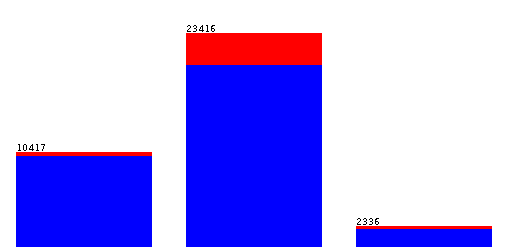
\includegraphics[width=0.8\textwidth]{pictures/contactHistogram.png}
  \caption{Histogram of the contact attribute}
  \label{fig:contactHistogram}
\end{figure}

\subsubsection{The Test Dataset}

\textbf{cworkPredict.arff} will be used to evaluate the best-performing models on the training dataset which will
be chosen using 10-fold cross validation. The number of clients in this dataset is 9042. 87.8\% of the clients
in this dataset did not subscribe to a term deposit, which is almost the same as the training set.

\section{Data Preprocessing}

The data provided for us was already split into a training dataset and an evaluation dataset. The test dataset
and the training dataset both have a similar proportion of clients who did not subscribe to a term deposit.

The numeric attributes in the dataset are age (a1), balance (a6), day (a10), duration (a12), campaign (a13), pdays (a14), 
and previous (a15). During the initial exploration of the dataset, we discovered that pdays (a14) and previous (a15) 
were very negatively skewed. Most clients also had a low / negative balance (a6) (see Figure ~\ref{fig:balanceHistogram}). 
These non-normal distributions may affect the naive Bayes classifier which assumes that numerical values have a normal 
distribution. To resolve this, we may need to discretise our numeric attributes. This will be tested when we train
our models by using preprocessing filters.

\begin{figure}[H]
  \centering
  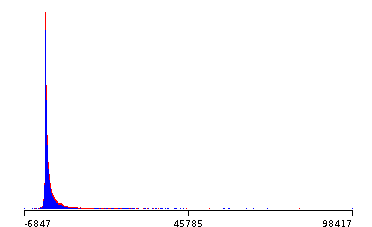
\includegraphics[width=0.8\textwidth]{pictures/balanceHistogram.png}
  \caption{Histogram of the balance attribute}
  \label{fig:balanceHistogram}
\end{figure}

\section{Classification Models}

We are now going to develop classification models using the training set and select the best performing models. This
will be carried out in five steps: benchmark models, attribute selection, model development, combining models, model selection,
and cost-based modelling.

\subsection{Benchmark Models}

The naive Bayes, k-nearest neighbour, J4.8, OneR, and logistic regression classifiers were applied with default parameters
and without any attribute preprocessing on the training dataset. This gave us a basic benchmark for each of these classifiers.
10-fold cross-validation was used to increase the reliability of our estimates. For the k-nearest neighbour classifier, 
we enabled the cross-validation option and set the kNN parameter to 10. The resulting value of k was 9.

\begin{table}[H]
  \begin{center}
    \begin{tabular}{r | r}
      Model & Accuracy  \\ \hline
      Naive Bayes & 88.1\% \\
      k-nearest neighbour (k = 9) & 89.2\% \\
      J4.8 & 90.4\% \\
      OneR & 88.5\% \\
      logistic regression & 90.2\% \\
    \end{tabular}
  \end{center}
  \caption{Basic benchmark results on training dataset}
  \label{tab:basicBenchmark}
\end{table}

\subsection{Attribute Selection}

In the data exploration stage, we determined that finding a subset of important attributes may help prevent overfitting.
Overfitting is when a model becomes too complex. It starts memorising data, including noise from the dataset. By reducing
the number of attributes used by the classification model, overfitting will hopefully by avoided.

\begin{itemize}
  \item{By visualising the decision tree of the J4.8 classifier, we can see that the duration (a12) attribute is at the
  root node}
  \item{Attribute selection using the CFS subset evaluator picked five attributes: marital (a3), housing (a7), loan (a8),
  duration (a12), poutcome (a16).}
  \item{Attribute selection using the information gain ranking filter ranked the attributes in the following order:
  duration (a12), poutcome (a16), pdays (a14), month (a11), contact (a9), age (a1), previous (a15), housing (a7),
  job (a2), day (a10), balance (a6), campaign (a13), loan (a8), education (a4), marital (a3), and default (a5).}
  \item{Attribute selection using the gain ratio feature evaluator ranked the attributes in the following order:
  poutcome (a16), duration (a12), pdays (a14), previous (a15), contact (a9), housing (a7), month (a11), age (a1),
  loan (a8), balance (a6), job (a2), campaign (a13), default (a5), day (a10), marital (a3), and education (a4).}
  \item{Attribute selection using the symmetrical uncertainty ranking filter ranked the attributes in the following order:
  duration (a12), poutcome (a16), pdays (a14), previous (a15), contact (a9), month (a11), housing (a7), age (a1), 
  balance (a6), job (a2), loan (a8), campaign (a13), day (a10), marital (a3), education (a4), default (a5).}
  \item{Attribute selection using the Chi-squared ranking filter ranked the attributes in the following order:
  duration (a12), poutcome (a16), pdays (a14), month (a11), age (a1), previous (a15), contact (a9), job (a2),
  housing (a7), day (a10), balance (a6), campaign (a13), education (a4), marital (a3), loan (a8), default (a5).}
\end{itemize}

All of these attribute evaluators agree that the two most important attributes are duration (a12) and poutcome (a16).
pdays (a14) is the third most important attribute according to all attribute evaluators apart from the CFS subset 
evaluator. Using these three attributes, the performance of the benchmark models is shown in Table ~\ref{tab:topThreeBenchmark}. 
Reducing the number of attributes to 3 improves the performance of the naive Bayes and the k-nearest neighbour classifiers. 
The performance of OneR remains unchanged and the performance of J4.8 and logistic regression is slightly reduced. 

\begin{table}[H]
  \begin{center}
    \begin{tabular}{r | r}
      Model & Accuracy  \\ \hline
      Naive Bayes & 89.1\% \\
      k-nearest neighbour (k = 9) & 89.7\% \\
      J4.8 & 90.1\% \\
      OneR & 88.5\% \\
      logistic regression & 90.0\% \\
    \end{tabular}
  \end{center}
  \caption{Benchmark results on three-attribute dataset}
  \label{tab:topThreeBenchmark}
\end{table}

The information gain ranking filter, the gain ratio feature evaluator, and the symmetrical uncertainty ranking
filter all have the same attributes in their top eight but in a different order. The Chi-squared ranking filter
also has seven of these eight attributes, with housing (a7), appearing in ninth place.
Because of this, we have determined an intermediate selection of eight attributes to be: 
duration (a12), poutcome (a16), pdays (a14), month (a11), contact (a9), age (a1), previous (a15), and housing (a7).
The performance of the classifiers with these eight attributes as seen in Table ~\ref{tab:topEightBenchmark} show
that increasing the number of attributes to eight slightly reduces the performance of the k-nearest neighbour
classifier. The performance of the J4.8 and the logistic regression classifiers are slightly increased. 

\begin{table}[H]
  \begin{center}
    \begin{tabular}{r | r}
      Model & Accuracy  \\ \hline
      Naive Bayes & 89.1\% \\
      k-nearest neighbour (k = 9) & 89.6\% \\
      J4.8 & 90.3\% \\
      OneR & 88.5\% \\
      logistic regression & 90.1\% \\
    \end{tabular}
  \end{center}
  \caption{Benchmark results on eight-attribute dataset}
  \label{tab:topEightBenchmark}
\end{table}

\subsection{Model Development}

During this phase, we experiment with each of our classifiers to enable us to select the most optimal parameters
for each model.

\subsubsection{Naive Bayes}

This model had the same performance on the three-attribute dataset and the eight-attribute dataset so we experimented 
with both datasets to determine the settings for the most optimal model. The naive Bayes classifier
assumes that numeric attributes have a normal distribution. During our initial data exploration, we discovered
that some attributes, namely pdays (a14) and previous (a15) were very negatively skewed. The balance (a6) attribute
also had a negatively skewed distribution but this attribute is not in the datasets used to train this model. The
easiest way to resolve this issue is to run the discretise filter. This will discretise numerical attributes into
a specified number of nominal bins.

Attributes in both datasets were discretised into 10 bins of equal frequency. For the three-attribute
dataset, the naive Bayes classifier achieved an accuracy of 89.3\%, a slight improvement when compared to the base benchmark.
An accuracy of 88.2\% was achieved by the naive Bayes classifier after discretising the eight-attribute dataset into
10 bins of equal frequency.

The three attribute dataset with 10 bins of equal frequency gives us the most accurate model for the naive Bayes
classifier. Table ~\ref{tab:naiveBayesBins} shows the accuracy of the naive Bayes classifier when different numbers of
bins are used on the discretise filter. 

\begin{table}[H]
  \begin{center}
    \begin{tabular}{r | r}
      Bins & Accuracy  \\ \hline
      5 & 89.2\% \\
      10 & 89.3\% \\
      15 & 89.4\% \\
      20 & 88.4\% \\
    \end{tabular}
  \end{center}
  \caption{Naive Bayes accuracy on the three-attribute dataset when the numerical attributes are discretised
  into a specified number of bins}
  \label{tab:naiveBayesBins}
\end{table}

These results show that for the naive Bayes classifier, you get the best performing model by using the three-attribute
dataset and discretising the numerical attributes into 15 bins of equal frequency.

\subsubsection{k-nearest Neighbour}

For this model, we continued to use 9 neighbours and the three-attribute dataset as the model performed best on this dataset.
We experimented with the distance weighting parameters and the results can be found in Table ~\ref{tab:kNNParams}

\begin{table}[H]
  \begin{center}
    \begin{tabular}{r | r}
      Weighting & Accuracy  \\ \hline
      No distance weighting & 89.7\% \\
      1/distance & 89.7\% \\
      1-distance & 89.7\% \\
    \end{tabular}
  \end{center}
  \caption{Results of varying the distance parameter}
  \label{tab:kNNParams}
\end{table}

As you can see in Table ~\ref{tab:kNNParams}, changing the distance weighting had no effect on the accuracy of this model.
No distance weighting needs to be done.

\subsubsection{J4.8}

For the J4.8 classifier, the key parameters to experiment with are the ones that control the complexity of the model.
These parameters are post-pruning, reduced error pruning, and minimum number of objects. J4.8 performed best with
all attributes so all of the experiments were carried out on the original training dataset (see Table ~\ref{tab:J48Params}).

\begin{table}[H]
  \begin{center}
    \begin{tabular}{l | r | r}
      Parameter & Parameter Value & Accuracy  \\ \hline
      Confidence Factor & 0.40 & 89.9\% \\
      Confidence Factor & 0.35 & 90.1\% \\
      Confidence Factor & 0.30 & 90.3\% \\
      Confidence Factor & 0.25 & 90.4\% \\
      Confidence Factor & 0.20 & 90.5\% \\
      Confidence Factor & 0.15 & 90.5\% \\
      Confidence Factor & 0.10 & 90.4\% \\
      Reduced error pruning (seed = 1) & True & 90.1\% \\
      Minimum number of objects  & 10 & 90.6\% \\
      Minimum number of objects  & 20 & 90.3\% \\
      Minimum number of objects  & 30 & 90.4\% \\
    \end{tabular}
  \end{center}
  \caption{Results of modifying J4.8 complexity parameters}
  \label{tab:J48Params}
\end{table}

The table above shows that the best performing model for this classifier is produced when the minimum number of objects
parameter is set to 10.

\subsubsection{OneR}

All of the benchmark models for the OneR classifier had the same performance for all attribute sets. This
is because the OneR classifier only uses one attribute for determining whether a client will subscribe to a term deposit
or not. So, to allow the classifier to choose the best attribute for itself, we will use the full attribute set to
further develop this model.

The OneR classifier discretises all numerical attributes into different buckets, similar to what the discretise 
attribute filter does. The classifier takes in a parameter, "minBucketSize", which specifies the minimum number of objects 
that must be in a bucket. In Table ~\ref{tab:OneRParams}, we experimented with this parameter and determined that a minimum
bucket size of 18 gives us the most accurate model.

\begin{table}[H]
  \begin{center}
    \begin{tabular}{r | r }
      Minimum Bucket Size & Accuracy  \\ \hline
      6 & 88.5\% \\
      8 & 88.6\% \\
      10 & 88.6\% \\
      12 & 88.7\% \\
      14 & 88.9\% \\
      16 & 89.2\% \\
      18 & 89.3\% \\
    \end{tabular}
  \end{center}
  \caption{Results of varying the minimum bucket size parameter}
  \label{tab:OneRParams}
\end{table}


\subsubsection{Logistic Regression}

The full training dataset gave us the best performance for this classifier so that is what we used.  This classifier uses
a ridge estimator and the ridge value is available for us to alter as a parameter. A smaller ridge parameter results
in a more flexible model. The results of experimenting with the ridge value are shown in Table ~\ref{tab:LogisticParams}

\begin{table}[H]
  \begin{center}
    \begin{tabular}{r | r }
      Ridge Value & Accuracy  \\ \hline
      $ 1 \times 10^{-8} $ & 90.2\% \\
      $ 1 \times 10^{-4} $ & 90.2\% \\
      $ 1 \times 1 $ & 90.2\% \\
      $ 1 \times 10 $ & 90.2\% \\
    \end{tabular}
  \end{center}
  \caption{Results of varying the ridge value}
  \label{tab:LogisticParams}
\end{table}

As you can see in Table ~\ref{tab:LogisticParams}, changing the ridge parameter did not alter the accuracy of the resulting
model in any meaningful way, so we decided to keep the ridge parameter at it's default setting ($ 1 \times 10^{-8} $)

\subsubsection{Voting Committee}

We now have five strongly performing models. All these models have an accuracy that is better than the default accuracy (88.4\%).
We combined all these models into a voting committee; all the models will vote on whether a client will subscribe to a term
deposit or not and the majority wins. The models chosen are naive Bayes with numerical attributes being discretised
into 15 bins of equal frequency, k-nearest neighbour with k set to 9, J4.8 with the minimum number of objects parameter set to 10,
OneR with the minimum bucket size parameter set to 18, and logistic regression with default parameters.

Because of the difficulties of using a different training set for different models in a voting committee, we decided to train
our models on the eight-attribute dataset. This dataset gives us the best performance for the naive Bayes and the OneR
classifiers. The performances of the other classifiers are only very slightly reduced on the eight attribute dataset when compared
to the optimal dataset for these classifiers.

After running the voting committee on the dataset with the best parameter settings for all five classifiers, t
he overall performance with 10-fold cross-validation was \textbf{90.0\%}. While this is pretty accurate, the
voting committee is still beaten by both the logistic regression model and the J4.8 model.

\subsubsection{Model Selection}

By experimenting with different classifiers and their parameters, we have determined that the J4.8 classifier with the minimum
number of objects parameter set to 10 produces the most accurate model. The J4.8 model has an estimated accuracy of 90.6\%
when using 10-fold cross-validation.

\subsection{Cost-based Modelling}

In this section, we ran all five models developed in the previous section using an unequal cross matrix. In the unequal
cost scenario specified by the banking institution, the cost of misclassifying a client who will subscribe to a term deposit
is 10 times that of misclassifying a client who will not. The cost matrix for this has the following structure:

\begin{table}[H]
  \begin{center}
    \begin{tabular}{l l }
      0.0 & 1.0 \\
      10.0 & 0.0 \\
    \end{tabular}
  \end{center}
  \label{tab:costMatrixStructure}
\end{table}

The default cost on the training set for a classifier that predicts that everyone will subscribe to a term deposit is equal
to the number of people that will not subscribe to a term deposit; 31981.

\subsubsection{Naive Bayes}

We ran the naive Bayes classifier with the three-attribute dataset and numerical attributes discretised into 15 bins
with the cost sensitive meta classifier. The naive Bayes model does give us estimates of class posterior
probabilities so we will run it with the minimise expected cost parameter set to true. This gave us the 
following confusion matrix:

\begin{table}[H]
  \begin{center}
    \begin{tabular}{l l }
      24791 & 7190 \\
      961 & 3227 \\
    \end{tabular}
  \end{center}
  \label{tab:naiveBayesCost}
\end{table}

The cost of this matrix is $ 7190 \times 1 + 961 \times 10 = 16800 $.

\subsubsection{k-nearest Neighbour}

We ran this classifier with the cost sensitive meta classifier, using the three-attribute dataset, 9 neighbours, 
and no distance weighting. Because the k-nearest neighbour classifier does not give us estimates of class posterior 
probability, we set the minimise expected cost parameter to false. This tells the meta classifier to reweigh 
the training instances using the cost matrix. This resulted in the following confusion matrix:

\begin{table}[H]
  \begin{center}
    \begin{tabular}{l l }
      23827 & 8154 \\
      962 & 3226 \\
    \end{tabular}
  \end{center}
  \label{tab:kNNCost}
\end{table}

The cost of this matrix is $ 8154 \times 1 + 962 \times 10 = 17704 $. This is more than the cost for naive Bayes.

\subsubsection{J4.8}
This classifier was ran with the cost sensitive meta classifier using the full training dataset and the minimum
number of objects parameter set to 10. Like k-nearest neighbour, this classifier does not give us estimates of
class posterior probabilities so we set the minimise expected cost parameter to false. This gave us the following
confusion matrix:

\begin{table}[H]
  \begin{center}
    \begin{tabular}{l l }
      26270 & 5711 \\
      485 & 3703 \\
    \end{tabular}
  \end{center}
  \label{tab:J48Cost}
\end{table}

The cost of this matrix is $ 5711 \times 1 + 485 \times 10 = 10561 $. This is the best cost so far.
margin.

\subsubsection{OneR}
For the OneR classifier, we used the full training set and set the minimum bucket size parameter to 18. This
classifier also does not give us estimates of class posterior probability so we set the minimise expected cost
parameter of the cost sensitive meta classifier to false. This gave us the following confusion matrix:

\begin{table}[H]
  \begin{center}
    \begin{tabular}{l l }
      20628 & 11353 \\
      990 & 3198 \\
    \end{tabular}
  \end{center}
  \label{tab:OneRCost}
\end{table}

The cost of this matrix is $ 11353 \times 1 + 990 \times 10 = 21253 $. This is the significantly worse than all
other costs.

\subsubsection{Logistic Regression}

We used the full training set again for this classifier with default parameters. Since this classifier does give
us posterior probabilities, we set the minimise expected cost parameter of the cost sensitive meta classifier
to true. The confusion matrix produced is shown below:

\begin{table}[H]
  \begin{center}
    \begin{tabular}{l l }
      25375 & 6606 \\
      514 & 3674 \\
    \end{tabular}
  \end{center}
  \label{tab:LogisticCost}
\end{table}

The cost of this matrix is $ 6606 \times 1 + 514 \times 10 = 11746 $. This is worse than the cost for the J4.8 model.
other costs.

\subsubsection{Model Selection}
From the results reported here, we can clearly see that the J4.8 model is the best for the unequal
cost problem. It significantly outperforms most of the other models, with only the logistic regression model
coming close. Because of this, it is not worth developing a voting model, the J4.8 model is clearly the way to go

\section{Conclusion}

In this section, we will evaluate our best model, the J4.8 classifier for both the equal cost and the unequal cost scenario,
on the test set. Then, I will talk about what I have learned by doing this coursework.

\subsubsection{Evaluation}
The accuracy of the J4.8 model with the minimum number of objects set to 10 on the test dataset with equal costs was 90.3\%.
This is pretty good, the accuracy of the default classifier on the test dataset 87.8\%. The confusion matrix on the test set
for this classifier was:

\begin{table}[H]
  \begin{center}
    \begin{tabular}{l l }
      7611 & 330 \\
      548 & 553 \\
    \end{tabular}
  \end{center}
  \label{tab:J48EqualTestCost}
\end{table}

Running the cost sensitive J4.8 model on the test set with unequal costs gave us the following confusion matrix:

\begin{table}[H]
  \begin{center}
    \begin{tabular}{l l }
      6510 & 1431 \\
      121 & 980 \\
    \end{tabular}
  \end{center}
  \label{tab:J48UnequalTestCost}
\end{table}

The total cost of this confusion matrix is $ 1431 \times 1 + 121 \times 10 = 2641 $. The cost of the default classifier
would be equal to the number of clients who would not subscribe to a term deposit; 7941. So as we can see, the cost
sensitive classifier performs very well on the test set. 

\subsubsection{What I have learned}
By doing this coursework, I have reinforced the knowledge I gained during the lectures on the way the different classifiers
work. I understand the preference to provide numerical attributes with a normal distribution for the naive Bayes classifier.
I strengthened my understanding of how other classifiers like the J4.8 classifier, the logistic regression classifier, and the
k-nearest neighbour classifier worked. Experimenting with the parameters of each of these classifiers gave me further insight
into their inner workings, especially when I experimented with the number of bins parameter for the J4.8 classifier. I could clearly
see how the J4.8 classifier discretises numerical attributes. I also grew an appreciation for simpler classifiers. The OneR
classifier, even though it only contains one rule, was able to keep up with other, more complex classifiers.

I am much more comfortable with using Weka. This coursework enabled me to experiment with the attribute selector, showing me
how to prune attributes which aren't very useful from a dataset. I also enjoyed creating a voting committee, I feel that
using a voting committee with a lot of similarly performing models may be a very strong option in some scenarios.

Finally, I was able to identify holes in my knowledge by doing this coursework. This enabled me to go through previous labs,
lectures, and online resources in order to reinforce my knowledge of machine learning and data mining.

\end{document}
